%%%%%%%%%%%%%%%%%%%%%%%%%%%%%%%%%%%%%%%%%
% University Assignment Title Page 
% LaTeX Template
% Version 1.0 (27/12/12)
%
% This template has been downloaded from:
% http://www.LaTeXTemplates.com
%
% Original author:
% WikiBooks (http://en.wikibooks.org/wiki/LaTeX/Title_Creation)
%
% License:
% CC BY-NC-SA 3.0 (http://creativecommons.org/licenses/by-nc-sa/3.0/)
% 
% Instructions for using this template:
% This title page is capable of being compiled as is. This is not useful for 
% including it in another document. To do this, you have two options: 
%
% 1) Copy/paste everything between \begin{document} and \end{document} 
% starting at \begin{titlepage} and paste this into another LaTeX file where you 
% want your title page.
% OR
% 2) Remove everything outside the \begin{titlepage} and \end{titlepage} and 
% move this file to the same directory as the LaTeX file you wish to add it to. 
% Then add \input{./title_page_1.tex} to your LaTeX file where you want your
% title page.
%
%%%%%%%%%%%%%%%%%%%%%%%%%%%%%%%%%%%%%%%%%
%\title{Title page with logo}
%----------------------------------------------------------------------------------------
%	PACKAGES AND OTHER DOCUMENT CONFIGURATIONS
%----------------------------------------------------------------------------------------

\documentclass[12pt]{article}
\usepackage[english]{babel}
\usepackage[utf8x]{inputenc}
\usepackage{amsmath}
\usepackage{graphicx}
\usepackage{subcaption}
\usepackage{float}
\usepackage[colorinlistoftodos]{todonotes}
\usepackage{hyperref}
\usepackage{algorithm2e}
\hypersetup{
    colorlinks = true,
    urlcolor= {violet}
}


\textheight=230truemm 
\textwidth=160truemm 
\hoffset=-10truemm \voffset=-20truemm

\begin{document}

\begin{titlepage}

\newcommand{\HRule}{\rule{\linewidth}{0.5mm}} % Defines a new command for the horizontal lines, change thickness here

\center % Center everything on the page
 
%----------------------------------------------------------------------------------------
%	HEADING SECTIONS
%----------------------------------------------------------------------------------------

\textsc{\LARGE Ukrainian Catholic University}\\[1cm] % Name of your university/college
\textsc{\Large  Faculty of Applied Sciences}\\[0.5cm] % Major heading such as course name
\textsc{\large Data Science Master Programme}\\[0.5cm] % Minor heading such as course title

%----------------------------------------------------------------------------------------
%	TITLE SECTION
%----------------------------------------------------------------------------------------
\vspace*{1cm}

\HRule \\[0.4cm]
{ \huge \bfseries Facial Expression Recognition in Natural Images}\\[10pt]
{\Large \bfseries Machine Learning final project progress report}\\[0.4cm] % Title of your document
\HRule \\[1cm]
 
%----------------------------------------------------------------------------------------
%	AUTHOR SECTION
%----------------------------------------------------------------------------------------
\vspace*{1cm}

% If you don't want a supervisor, uncomment the two lines below and remove the section above
\Large \emph{Authors:}\\
Anastasiia \textsc{Khaburska}\\Andrii \textsc{Yurkiv}\\[1cm] % Your name

%----------------------------------------------------------------------------------------
%	DATE SECTION
%----------------------------------------------------------------------------------------
\vspace*{1cm}
{\large 27 April 2019}\\[2cm] % Date, change the \today to a set date if you want to be precise

%----------------------------------------------------------------------------------------
%	LOGO SECTION
%----------------------------------------------------------------------------------------

\includegraphics[height=5cm]{UCU-Apps.png}\\[1cm] % Include a department/university logo - this will require the graphicx package
 
%----------------------------------------------------------------------------------------

\vfill % Fill the rest of the page with whitespace

\end{titlepage}


% \begin{abstract}
	
% \end{abstract}

\section{Introduction}

Facial expression is one or more motions or positions of the muscles beneath the skin of the face. These movements convey the emotional state of an individual and become the primal form of nonverbal communication.\\

It is assumed that certain facial expressions and gestures correspond to specific emotions (for instance, happiness is associated with laughter and smiling, sadness with tears, anger with clenched jaw, fear with grimace, surprise with raised eyebrows and wide eyes and disgust with wrinkled nose and squinted eyes) which  are recognized by humans regardless of culture, language or time. But in general, this hypothesis has not been scientifically verified and received both critical and supportive reviews.\\

Both sides of this scientific debate agree that the face expresses emotion. The controversy surrounds the uncertainty about what specific emotional information is read from a facial expression \cite{wiki}.


\section{Motivation}

It has been proved multiple times that the majority of information human perceives (up to $83\%$) during message absorption is obtained through eyesight. For this purpose body language in general, and facial expression, in particular, are the things which provide the most essential and specific information about the intentions and emotional state of the message source.\\

It's not hard to conclude that accurate perception of facial expressions is a key to effective face-to-face communication.\\

Humans have a great ability to perform this kind of tasks. And since main facial expressions are universal and do not vary with culture or environment, we usually recognize others emotional state pretty well (at least when our interlocutors are not intentionally hiding it).\\

\begin{figure}
	\centering
	\includegraphics[width=\textwidth]{../images/t-sne-visualization.png}
	\caption{Visualization of 400 random images from \texttt{fer2013} data set using $t$-SNE algorithm}
	\label{fig:tsne}
\end{figure}

But for a machine, it is not an easy task. We tried to visualize images in two-dimensional space using $t$-SNE algorithm [\ref{fig:tsne}]. As you can observe, facial expressions are not the things that the algorithms uses to differentiate between images. It is skin color, age gender what algorithm notices.\\

If we asked any human to take a a look on faces (for example, those [\ref{fig:faces}]) and say whether there is a substantial visual difference between them, we would certainly hear "yes". But, in fact, they are not that different. It is our ability to recognize these differences that makes humans consider them substantial. In general, there are few reasons why machine learning model usually perform much worse compared to humans in recognizing facial expressions (while outperforming in other classification tasks):

\begin{itemize}
    \item 
    Humans do not perceive facial expressions separately from other parts of body language. For facial expressions, context is very important, because it provides a great deal of additional information.
    \item
    Regardless of their universality, facial expressions are very diverse and vary substantially due to the race, age, gender, nationality and culture.
    \item 
    People are brilliant at determining how they feel. But in some cultures, it is normal to hide your real emotions behind the neutral or happy facial expression. It is especially distinguishable in western cultures, where excessive emotionality is not considered as an element of effective communication. Machine learning model doesn't have this prior knowledge and hence use a generalized approach to cases where cultural nuances are crucial.
    \item 
    Some kinds of facial expressions are very similar (for example, without context, it's hard to distinguish surprise from fear, or sadness from neutrality). And image similarity is a fundamental property when the model is trying to determine class depicted on it. The model fails to generalize well and makes mistakes by focusing on the wrong features.
\end{itemize}



In this project, we investigated deep learning approaches to the task of facial expression recognition and  developed an end-to-end machine learning system of facial expression recognition in natural images. It consists of two parts: a face detector and expression recognizer. Unfortunately, we haven't found a data set to evaluate our end-to-end system (we need a data set that contains images with faced in different contexts labelled with facial expression classes). So, we evaluated our results in conjunction with state-of-the-art performance on \texttt{fer2013} data set, which is equal to $75.2\%$

\section{Related Work}

Byoung Chul Ko in a paper “A Brief Review of Facial Emotion Recognition Based on Visual Information”\cite{FERreview} gives an overview of researches in the field of FER conducted over the past decades. To tackle the problem of FER researchers tried such techniques : 
\begin{enumerate}
\item Conventional  FER  approaches along the  representative categories of FER systems and their main algorithms. 
\item Deep-learning-based FER approaches
\item Hybrid deep-learning approach combining a convolutional neural network (CNN)for the spatial features of an individual frame and long short-term memory (LSTM) for temporal features of consecutive frames.
\end{enumerate}

Papers in this area are usually focused on recognizing human emotion in the context of video data (consecutive frames)\cite{video1}. In terms of this homework project we investigated deep-learning-based approaches, that solve the problem for from still images (individual frames). An overview to various deep learning methods applicable to this particular problem was also made by Alexandru Savoiu and James Wong in \cite{deepNN}. Our contribution was to learn and implement different approaches, create own models, train them on the conjoint data-set, evaluate and then compare.

\section{Project idea. Data}

The project idea was inspired by Kaggle competition "Challenges in Representation Learning: Facial Expression Recognition Challenge". It was organized in 2013, but we think that the topic is still relevant today. The \texttt{fer2013} data set \cite{dataset} for this competition was prepared by Pierre-Luc Carrier and Aaron Courville.\\

\begin{figure}
	\centering
	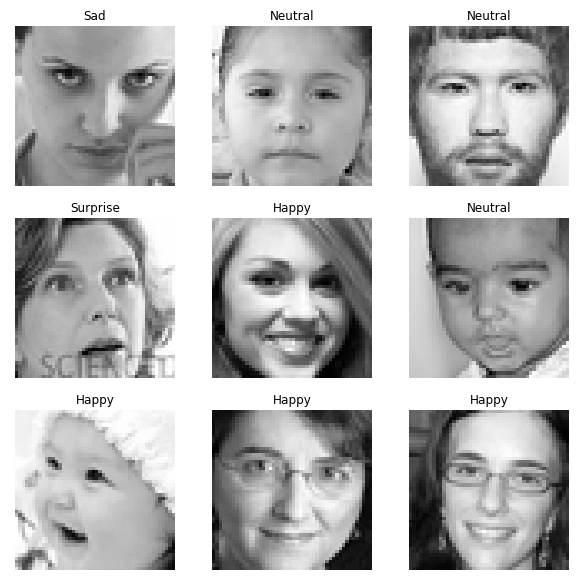
\includegraphics[width=0.5\textwidth]{../images/examples.png}
	\caption{Examples of images from \texttt{fer2013} data set}
	\label{fig:faces}
\end{figure}

The \texttt{fer2013} data set consists of $48\times48$ pixel gray-scale images of faces. The faces have been automatically registered so that the face is more or less centered and occupies about the same amount of space in each image. The task is to categorize each face based on the emotion shown in the facial expression into one of seven categories (0=Angry, 1=Disgust, 2=Fear, 3=Happy, 4=Sad, 5=Surprise, 6=Neutral).\\

The data set is divided into train, validation and test splits. The training set consists of $28,709$ examples. The validation set consists of $3,589$ examples. The final test set consists of another $3,589$ examples.\\

\begin{table}[H]
	\centering
	\begin{tabular}{ | l | l | l | l | l | }
		\hline
		Expression & Train & Validation & Test & \% of samples \\ \hline
		Angry & 3995 & 467 & 491 & 13.8 \\ %\hline
		Disgust & 436 & 56 & 55 & \textbf{1.52} \\ %\hline
		Fear & 4097 & 496 & 528 & 14.27 \\ %\hline
		Happy & 7215 & 895 & 879 & \textbf{25.05} \\ %\hline
		Neutral & 4965 & 607 & 626 & 17.27 \\ %\hline
		Sad & 4830 & 653 & 594 & 16.93 \\ %\hline
		Surprise & 3171 & 415 & 416 & 11.15 \\ 
		\hline
	\end{tabular}
	\caption{Distribution of classes in the data set.}
\end{table}

The classes in the data set are not well-balanced. First of all, we have highly underrepresented \texttt{Disgust} class. Also, $25.05\%$ of samples correspond to the \texttt{Happy} class, which is more than the fraction of \texttt{Angry} and \texttt{Surprise} altogether ($24.95\%$).\\ 

This imbalance issue imposes additional activities in our development process:

\begin{itemize}
    \item 
    We performed data augmentation in order to make it more robust.
    \item
    We used minibatch normalization, to reduse the covarianse shift and to increase training rates.
    \item
    As an evaluation metric, we used the confusion matrix to determine the weaknesses of the model and possible improvement strategies.
\end{itemize}

Besides the imbalance, \texttt{fer2013} data set contains trash samples (which do not contain a face) and several misclassified examples. These imperfections make the classification harder because the model has to generalise well and be robust to incorrect data. 

% To address this problem and clean the dataset we used our first part of solution -- face recognition. 




\section{Approach to the solution}
\subsection{Face detection}

 Since we haven't found a data set on which we can assess both face detection and facial recognition models performance we decided to use pretrained Haar Cascade model for front-face detection from \texttt{cv2} python module. It works well in general but sometimes fails to detect faces in unusual conditions or under unusual aspect. But it is absolutely fine if we take into account the scope and setting of our project.\\

\subsection{Baseline model}

Our baseline facial expression recognition model is a 4-layer CNN with 3 dense layers. The model architecture is visualized in [\ref{fig:baseline}].\\

On each layer except output one we used ReLU activation function. On the output layer we used Softmax function. We applied batch normalization after each convolutional layer in order to make our model converge faster and omit getting stuck in local minima. Besides it, we applied the Dropout regularization technique at each layer to prevent overfitting and make our model generalize better. \\

\begin{figure}
	\centering
	\includegraphics[width=\textwidth]{../images/baseline-architecture.png}
	\caption{Baseline model architecture}
	\label{fig:baseline}
\end{figure}

\subsection{Baseline model with data augmentation}

As we mentioned in the previous section, the data set we were training our model on was very unbalanced. We decided to tackle this problem using data augmentation for train set. The general approach was as following: we randomly augmented $100\%$ of \texttt{Disgust} class images, $50\%$ of \texttt{Fear} and \texttt{Angry} classes and $10\%$ of \texttt{Surprise}, \texttt{Happy}, \texttt{Neutral} and \texttt{Sad} ones. We used 5 different augmentation techniques for each image: horizontal flipping, left/right rotation by $15$ degrees, noise and blur introduction. As a result, we increased our train set size by $32490$ images. Our baseline model was simple enough to handle this amount of data without substantial increase in training time.\\

We didn't apply data augmentation for modification of VGG-19 and Original VGG-19, because it would take much longer time to train those models with $2\times$ more data.\\ 

Data augmentation increased the performance of the baseline model by nearly $3\%$, which means that it was a reasonable procedure to perform. One important thing to note is it was crucial for the model that dropout rate at each layer was equal to $0.5$. Otherwise model over-fitted and performed poorly on test data.\\

\subsection{Baseline model with HOG}

During data analysis stage of our project we had an idea that introduction of additional features to the model could increase its performance. There are a lot of ways to extract additional information from the image. In our setting the most applicable were Face Landmarks and HOG (Histogram of Oriented Gradients). Each of them employs different approach to feature extraction and, hence, results in different amount of features. For example, using Face Landmarks, we usually get less than 100 features, and using HOG we can get up to $n\times n$ features (where $n$ is image height).\\

Observing results obtained in \cite{githubHOG}, we came to conclusion that HOG features/Face Landmarks do not considerably improve the model performance in our problem setting. But we still decided to check this assumption.\\

When choosing among Face Landmarks and HOG we chose second one, because it is much easier to implement. We added a branch with HOG input to baseline model, and trained it on the regular data without augmentation. The model obtained performed really poorly (accuracy decreased by $4\%$) and consequently we decided not to use additional features in the future modeling process.

\subsection{AlexNet model}

One more model we tried was an adaptation of classic AlexNet model. This model consists of 6 convolutional layers and 4 dense layers. ReLU activation function was used on each layer expcept the output one, where Softmax is employed. In order to simplify this model we decreased the number of neurons in the dense layers (first - by half, second - by $3/4$ and third - by half). Besides it, we had to decrease kernels and pooling size in the first layers of the network, since the original model was developed for $224\times 224$ images, and our images are much smaller.\\

The AlexNet model architecture is depicted in [\ref{fig:alexnet}].\\

\begin{figure}
	\centering
	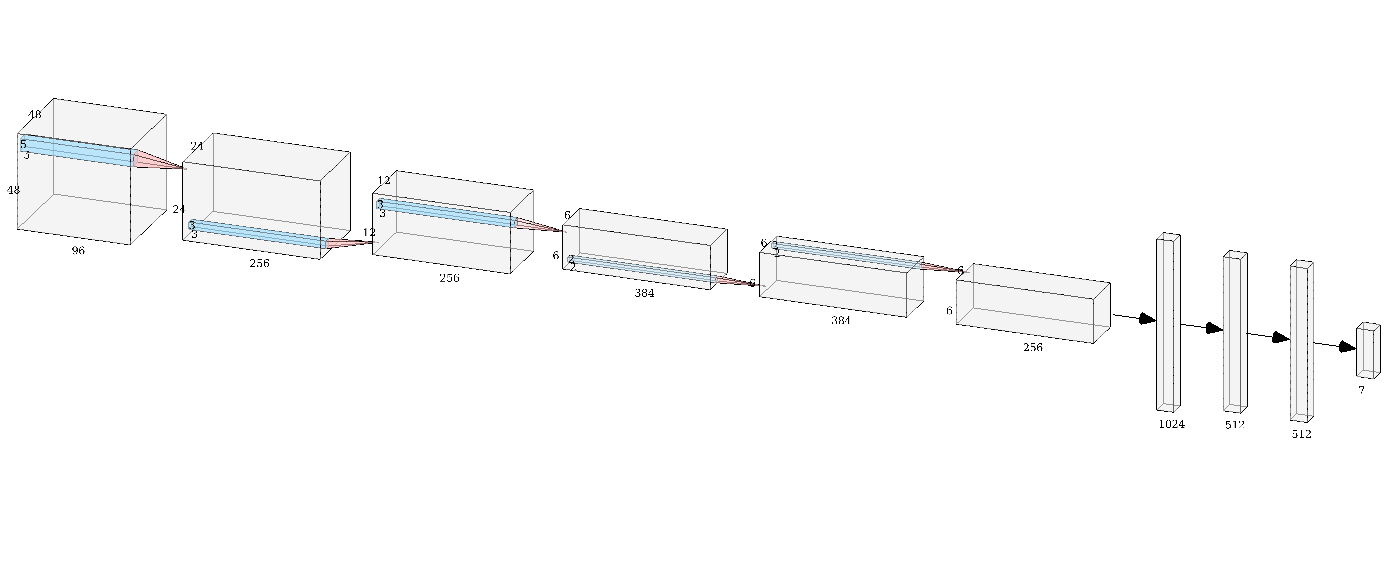
\includegraphics[width=\textwidth]{../images/alexnet-architecture.png}
	\caption{AlexNet model architecture}
	\label{fig:alexnet}
\end{figure}

AlexNet model proved to perform worse than the baseline in both regular and augmented train set settings.

\subsection{VGG-19 model}

The original VGG network described in ~\cite{VGG} uses an architecture with very small (5x5; 3x3) convolution filters, consecutively with depth 64, 128, 256, 512, pushing size up to 19, depending on the problem. This architecture showed sufficient accuracy for large scale RGB images classification tasks.\\

We adjusted VGG network for images of size $48\times48\times1$. During training, the best result of 66.5\% accuracy was obtained with 7-layer VGG network. The architecture of this adjusted VGG network is shown in [\ref{fig:VGG}]. The only preprocessing we did was image scaling to range [0:1] by division of each pixel pixel by 255. Then image is passed through the convolutional layer, with receptive field of size $5\times5$, and then through  stack of convolutional layers, where we use filters with a very small receptive field 3x3 (which is the smallest size to capture the notion of left/right, up/down, center ~\cite{VGG}). The convolution stride is fixed to 1 pixel and the padding is adjusted in a way that after each convolution the size of the image remains the same. Also, for downsampling only the important features of the images, as in ~\cite{MaxOut}, we decided to add MaxPooling after the first convolution and the Average Pooling after the each second convolution. Each pooling reduces the height and length of the layer by two. To prevent overfitting even more, as suggested in ~\cite{DropOut} and ~\cite{DropOutOverfit}, we decided to use dropout in all layers with a fraction 0.5.\\

On each layer except output one we used ReLU activation function.  On the output layer we used Softmax function. To adress the problem of internal covariance shift, we performed the normalization for each training mini-batch. Batch Normalization also acts as a regularizer and achieves the same accuracy with fewer training steps ~\cite{batchnormalization}.

\begin{figure}
	\centering
	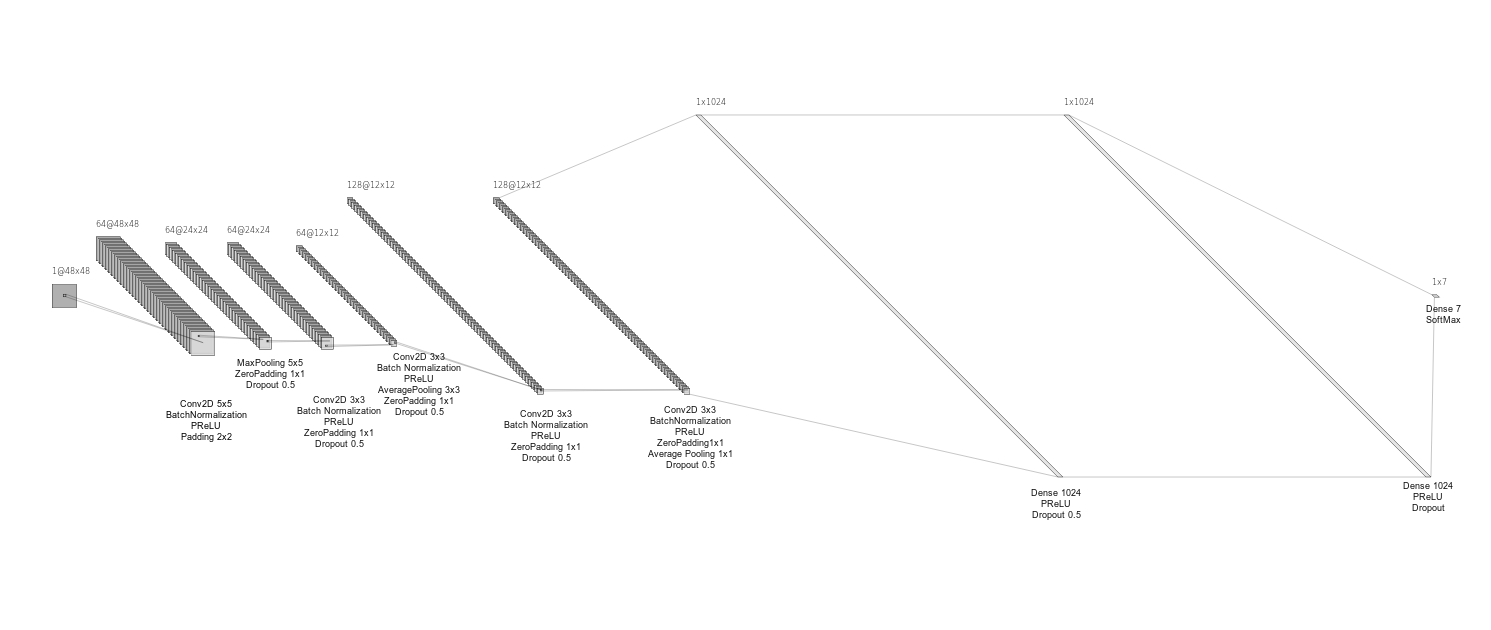
\includegraphics[width=\textwidth]{../images/vgg-adjusted.jpg}
	\caption{Customized VGG model architecture}
	\label{fig:VGG}
\end{figure}

\subsection{Ensamble approach}

The models we trained (even the best ones) showed pretty mediocre results on the test set, comparing to the state-of-the-art models proposed, for example in \cite{ferSOTA}. In this specific paper authors achieved astonishing accuracy of $75.2\%$ using ensemble of 8 complex models (VGG, ResNet and Inception). We decided that this approach would be reasonable in our setting as well.\\

We tried 2 different ensembles: combinations of 3 strongest models (in our case - Baseline with Augmentation, VGG and Original VGG) and combination of 5 strongest models (those used in previous ensemble plus Baseline and Alexnet with Augmentation). As a result we got a substantial increase in accuracy for both validation and test sets. As expected, ensemble of 5 models performed better than the ensemble of 3. \\

For the ensemble of 5 models we have used "smart" voting system by weighting models' votes using their validation accuracy. It was very beneficial in those cases when two models predicted one class and two - the other one. This approach allowed us to fight ambiguity and let better models to make the decision.\\

\subsection{Training}

We trained our models for different number of epochs depending on such parameters as crossentropy loss and categorical accuracy. We tried different approaches and tuned hyper parameters many times in order to make our models more robust (we changed learning rates, dropout rates, added/removed layers, decreased their size, changed optimizers and enhanced existing models with augmented data). Besides it, we always reused pretrained weights in the future iterations to accelerate computations and iterate faster.\\

It should be noted that validation loss didn't fall below 0.97 in any of our experiments. During the training process it usually oscillated around 1 and then, after large number of epochs began to slowly but gradually increase till the end of the training. We tried a lot of things to change this behaviour, but didn't succeed.

\section{Evaluation}

The accuracies of the model used can be seen in \ref{table:acc}. Two types of models performed best in the FER task: simple models trained on aggressively augmented training data (BaseAug) and complex models trained on regular training data. Those models, that were somewhat in the middle (AlexNet) didn't really performed well. We explain it by the specificity of the task. Simple model (shallow, if we are talking about CNN) doesn't have an ability to learn comoplex hypothesis. That's why it benefits a lot from augmented data. Complex, deep CNN models, on the other hand, have this ability, so they can perform well even without data augmentation.\\

As we can observe from the confusion matrix [\ref{fig:conf}], constructed using predictions of ensemble of 5 models, it does a great job recognizing \texttt{Happy} and \texttt{Surprise} expressions, while failing to recognize accurately such expressions as \texttt{Fear}, \texttt{Sad} and \texttt{Angry}. In general, it's not an unexpected result. Those are complex and ambiguous facial expressions that are often misinterpreted if seen without corresponding context. 

\begin{table}[H]
	\centering
	\begin{tabular}{ | l | l | l | l | l | l | l | l | l | }
		\hline
		 & Base & BaseAug & Alex & AlexAug & VGG & VGG-O & E3 & E5 \\ 
		\hline
		Validation & 0.636 & 0.655 & 0.616 & 0.635 & 0.646 & 0.662 & 0.668 & \textbf{0.681} \\
		Test & 0.642 & 0.672 & 0.635 & 0.643 & 0.670 & 0.675 & 0.693 & \textbf{0.703} \\ 
		\hline
	\end{tabular}
	\caption{Performance of the models and ensembles. Base: Baseline, BaseAug: Baseline with Augmentation, Alex: AlexNet, AlexAug: AlexNet with Augmentation, VGG: Modified VGG, VGG-O: Original VGG, E3: Ensemble of 3 strongest models, E5: Ensemble of 5 strongest models}
	\label{table:acc}
\end{table}

\begin{figure}
	\centering
	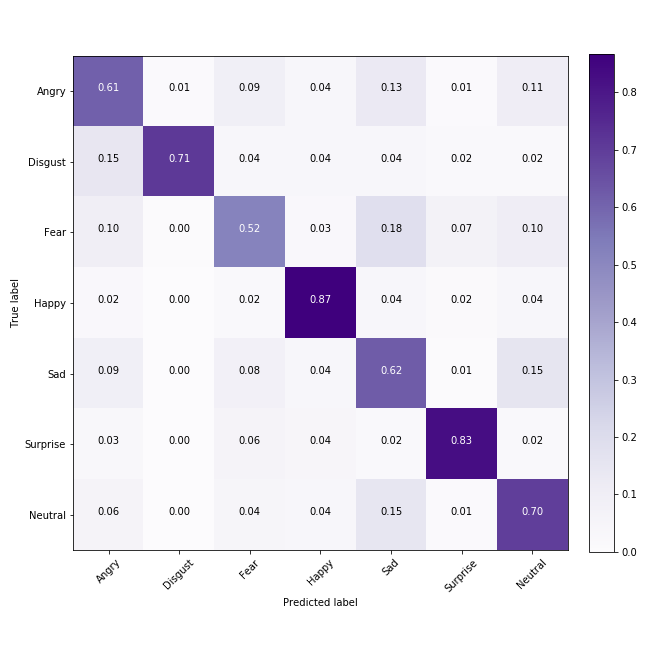
\includegraphics[width=0.65\textwidth]{../images/confusion.png}
	\caption{Normalized confusion matrix}
	\label{fig:conf}
\end{figure}

\section{Conclusions}

As a result of this project, we developed an efficient end-to-end system for facial expression recognition in natural images. We didn't succeed to achieve state-of-the-art accuracy on the data set, but still obtained performance that would provide us second absolute place in the original Kaggle leaderboard ($70.3\%$).\\

Our final solution for classification problem is an ensamble of 5 models: baseline CNN model, baseline model trained on augmented data, AlexNet model trained on augmented data,  modified VGG network and Original VGG network. This is not the fastest or most efficient solution, but it generalizes well. \\

During the project implementation we made some important observations:

\begin{itemize}
	\item 
	Facial expressions are really hard to recognize. They are subtle, ambiguous and culture-specific. It's impossible to create a perfect classifier without additional contextual information.
	\item 
	Complex CNN models (like VGG) really worth it. They may be hard to train or store, but at the same time they are able to learn highly complex non-linear hypothesis which gives them considerable advantage over simpler models. 
	\item 
	HOG doesn't worth it (at least in this problem). Facial expressions are too complex and subtle to be noticed by HOG, and as a result it just introduces unnecessary noise which doesn't make the model perform better.
	\item 
	Data augmentation is a very reasonable way to improve your model and make it generalize better by smoothing data imbalance. Other important question is what and how to augment, especially in cases when two classes are very similar (\texttt{Sad} and \texttt{Neutral} in our case).
	\item 
	If you hit the ceiling with separate models, try ensemble. It will for sure make your model to perform better.
	\item 
	Computational resources are very important. They allow to iterate faster and to implement you idea in hours instead of days. 
	\item
	There is no need to implement existing things from scratch if you want to move fast. In our case, for example, face detection problem was solved long time ago (it is even a part of existing python package), so we decided not to concentrate on it.
\end{itemize}



The code, experiments and scripts can be found in project GitHub repository:\\ 

\url{https://github.com/andreyurkiv/facial-expression-recognition}.




\newpage
\begin{thebibliography}{6}
	\bibitem{dataset} 
	I. Goodfellow et al.
	\textit{Challenges in Representation Learning: A report on three machine learning contests.}\\
	\url{https://arxiv.org/pdf/1307.0414.pdf}
	
	\bibitem{wiki}
	Wikipedia contributors
	\textit{Facial expression {Wikipedia}{,} The Free Encyclopedia.}\\
	\url{https://en.wikipedia.org/w/index.php}
	
	\bibitem{FERreview}
	B. C. Ko
	\textit{A Brief Review of Facial Emotion Recognition Based on Visual Information.}\\
	\url{https://pdfs.semanticscholar.org/1e7a/e86a78a9b4860aa720fb0fd0bdc199b092c3.pdf}
	
	\bibitem{video1}
	S.Kahou, C. Pal, X. Bouthillier, P.  Froumenty,  C. Gulcehre,  R.  Memisevic, P.  Vincent,  A.  Courville,  Y.  Bengio.
	\textit{Combining Modality Specific Deep Neural Networks for Emotion Recognition in Video.}\\
	\url{http://www.professeurs.polymtl.ca/christopher.pal/icmi2013/icmi2013_grand_challenge_winner.pdf}
	
	\bibitem{video2}
	T. Le.
	\textit{Applying Artificial Neural Networks for Face Recognition.}\\
	\url{https://www.researchgate.net/publication/258380240_Applying_Artificial_Neural_Networks_for_Face_Recognition}
	
	\bibitem{deepNN}
	A. Savoiu, J. Wong.
	\textit{Recognizing Facial Expressions Using Deep Learning.}\\
	\url{http://cs231n.stanford.edu/reports/2017/pdfs/224.pdf}
	
	\bibitem{VGG}
	K. Simonyan, A. Zisserman. 
	\textit{Very deep convolutional networks for large-scale image recognition.}\\
	\url{https://arxiv.org/pdf/1409.1556.pdf}
	
	\bibitem{batchnormalization}
	S. Ioffe, C. Szegedy.
	\textit{Batch Normalization: Accelerating Deep Network Training by Reducing Internal Covariate Shift.}\\
	\url{https://arxiv.org/pdf/1502.03167v3.pdf}
	
	\bibitem{MaxOut}
	I. J. Goodfellow, D. Warde-Farley, M. Mirza, A. C.Courville, and Y. Bengio.
	\textit{Maxout Networks.}\\
	\url{https://arxiv.org/pdf/1302.4389.pdf}
	
	\bibitem{DropOut}
	Stefan Wager,  Sida Wang and Percy Liang.
	\textit{Dropout Training as Adaptive Regularization.}\\
	\url{https://arxiv.org/pdf/1307.1493.pdf}
	
	\bibitem{DropOutOverfit}
	N. Srivastava, G. Hintonhinton, A. Krizhevskykriz, I. Sutskeverilya, R. Salakhutdinov.
	\textit{Dropout:  A Simple Way to Prevent Neural Networks from Overfitting.}\\
	\url{http://jmlr.org/papers/volume15/srivastava14a/srivastava14a.pdf}

    \bibitem{githubHOG}
    A. Horseman
    \textit{Facial expression recognition using CNN in Tensorflow}\\
    \url{https://github.com/amineHorseman/facial-expression-recognition-using-cnn}

    \bibitem{alexnet}
    A.Krizhevsky, I. Sutskever, G. Hinton
    \textit{ImageNet Classification with Deep Convolutional Neural Networks}\\
    \url{https://papers.nips.cc/paper/4824-imagenet-classification-with-deep-convolutional-neural-networks.pdf}
    
    \bibitem{ferSOTA}
    C. Pramerdorfer, M. Kampel
    \textit{Facial Expression Recognition using Convolutional Neural Networks: State of the Art}\\
    \url{https://arxiv.org/pdf/1612.02903.pdf}
    

\end{thebibliography}

\newpage
\appendix
\section{Appendix}

\begin{figure}[h]
	\centering
	\begin{subfigure}[h]{0.65\textwidth}
		\includegraphics[width=\textwidth]{../data/original/test2.jpg}
		\caption{Original image}
	\end{subfigure}\qquad
	\begin{subfigure}[h]{0.65\textwidth}
		\includegraphics[width=\textwidth]{../images/test2_labeled.jpg}
		\caption{Predicted facial expressions}
	\end{subfigure}
	\caption{Baseline model results}
\end{figure}


\end{document}